%% USPSC-modelo-ICMCp.tex
% ---------------------------------------------------------------
% USPSC: Modelo de Trabalho Academico (tese de doutorado, dissertacao de
% mestrado e trabalhos monograficos em geral) em conformidade com 
% ABNT NBR 14724:2011: Informacao e documentacao - Trabalhos academicos -
% Apresentacao
%----------------------------------------------------------------
%% Esta é uma customização do abntex2-modelo-trabalho-academico.tex de v-1.9.5 laurocesar 
%% para as Unidades do Campus USP de São Carlos:
%% EESC - Escola de Engenharia de São Carlos
%% IAU - Instituto de Arquitetura e Urbanismo
%% ICMC - Instituto de Ciências Matemáticas e de Computação
%% IFSC - Instituto de Física de São Carlos
%% IQSC - Instituto de Química de São Carlos
%%
%% Este trabalho utiliza a classe USPSC.cls que é mantida pela seguinte equipe:
%% 
%% Coordenação e Programação:
%%   - Marilza Aparecida Rodrigues Tognetti - marilza@sc.usp.br (PUSP-SC)
%%   - Ana Paula Aparecida Calabrez - aninha@sc.usp.br (PUSP-SC)
%% Normalização:
%%   - Brianda de Oliveira Ordonho Sigolo - brianda@usp.br (IAU)
%%   - Eduardo Graziosi Silva - edu.gs@sc.usp.br (EESC)
%%   - Eliana de Cássia Aquareli Cordeiro - eliana@iqsc.usp.br (IQSC)
%%   - Flávia Helena Cassin - cassinp@sc.usp.br (EESC)
%%   - Maria Cristina Cavarette Dziabas - mcdziaba@ifsc.usp.br (IFSC)
%%   - Regina Célia Vidal Medeiros - rcvmat@icmc.usp.br (ICMC)
%%
%% O USPSC-modelo.tex e USPSC-TCC-modelo.tex utilizam diversos arquivos relacionado em 
%% 2.1 Pacote USPSC: Classe USPSC e modelos de trabalhos acadêmicos	do Tutorial do Pascote 
%%  USPSC para modelos de trabalhos de acadêmicos em LaTeX - versão 3.1


%----------------------------------------------------------------
%% Sobre a classe abntex2.cls:
%% abntex2.cls, v-1.9.5 laurocesar
%% Copyright 2012-2015 by abnTeX2 group at https://www.abntex.net.br/ 
%%
%----------------------------------------------------------------

\documentclass[
% -- opções da classe memoir --
12pt,		% tamanho da fonte
openright,	% capítulos começam em pág ímpar (insere página vazia caso preciso)
twoside,  % para impressão em anverso (frente) e verso. Oposto a oneside - Nota: utilizar \imprimirfolhaderosto*
%oneside, % para impressão em páginas separadas (somente anverso) -  Nota: utilizar \imprimirfolhaderosto
% inclua uma % antes do comando twoside e exclua a % antes do oneside 
a4paper,			% tamanho do papel. 
% -- opções da classe abntex2 --
chapter=TITLE,		% títulos de capítulos convertidos em letras maiúsculas
% -- opções do pacote babel --
english,			% idioma adicional para hifenização
french,				% idioma adicional para hifenização
spanish,			% idioma adicional para hifenização
brazil				% o último idioma é o principal do documento
% {USPSC-classe/USPSC} configura o cabeçalho contendo apenas o número da página
]{USPSC-classe/USPSC}
%]{USPSC-classe/USPSC1}
% Inclua % antes de ]{USPSC-classe/USPSC} e retire a % antes de %]{USPSC-classe/USPSC1} para utilizar o 
% cabeçalho diferenciado para as páginas pares e ímpares:
%- páginas ímpares: com seções ou subseções e o número da página
%- páginas pares: com o número da página e o título do capítulo 
% ---
% ---
% Pacotes básicos - Fundamentais 
% ---
\usepackage[T1]{fontenc}		% Seleção de códigos de fonte.
\usepackage[utf8]{inputenc}		% Codificação do documento (conversão automática dos acentos)
\usepackage{lmodern}			% Usa a fonte Latin Modern
% Para utilizar a fonte Times New Roman, inclua uma % no início do comando acima  "\usepackage{lmodern}"
% Abaixo, tire a % antes do comando  \usepackage{times}
%\usepackage{times}		    	% Usa a fonte Times New Roman	
% Para usar a fonte , lembre-se de tirar a % do comando %\renewcommand{\ABNTEXchapterfont}{\rmfamily}, localizado mais abaixo, logo após "Outras opções para nota de rodapé no Sistema Numérico" 				
\usepackage{lastpage}			% Usado pela Ficha catalográfica
\usepackage{indentfirst}		% Indenta o primeiro parágrafo de cada seção.
\usepackage{color}				% Controle das cores
\usepackage{graphicx}			% Inclusão de gráficos
\usepackage{float} 				% Fixa tabelas e figuras no local exato
\usepackage{chemfig,chemmacros} % Para escrever reações químicas
\usepackage{tikz}				% Para escrever reações químicas e outros
\usetikzlibrary{positioning}
\usepackage{microtype} 			% para melhorias de justificação
\usepackage{pdfpages}
\usepackage{makeidx}            % para gerar índice remissivo
\usepackage{hyphenat}          % Pacote para retirar a hifenizacao DO TEXTO
\usepackage[absolute]{textpos} % Pacote permite o posicionamento do texto
\usepackage{eso-pic}           % Pacote para incluir imagem de fundo
\usepackage{makebox}           % Pacote para criar caixa de texto
% ---

% ---
% Pacotes de citações
% Citações padrão ABNT
% ---
% Sistemas de chamada: autor-data ou numérico.
% Sistema autor-data
\usepackage[alf, abnt-emphasize=bf, abnt-thesis-year=both, abnt-repeated-author-omit=no, abnt-last-names=abnt, abnt-etal-cite, abnt-etal-list=3, abnt-etal-text=it, abnt-and-type=e, abnt-doi=doi, abnt-url-package=none, abnt-verbatim-entry=no]{abntex2cite}
%\bibliographystyle{USPSC-classe/abntex2-alf-USPSC}
% Se o idioma for o inglês, inclua % no comando acima e exclua o % do comando abaixo
\bibliographystyle{USPSC-classe/abntex2-alfeng-USPSC}

% Para o IQSC, que indica todos os autores nas referências, incluir % no início dos comandos acima e retirar a % dos comandos abaixo 
%\usepackage[alf, abnt-emphasize=bf, abnt-thesis-year=both, abnt-repeated-author-omit=no, abnt-last-names=abnt, abnt-etal-cite, abnt-etal-list=0, abnt-etal-text=it, abnt-and-type=e, abnt-doi=doi, abnt-url-package=none, abnt-verbatim-entry=no]{abntex2cite} 
%\bibliographystyle{USPSC-classe/abntex2-alf-USPSC}
% Se o idioma for o inglês, exclua % no comando acima ou do comando abaixo
%\bibliographystyle{USPSC-classe/abntex2-alfeng-USPSC}

% Sistema Numérico
% Para citações numéricas, sistema adotado pelo IFSC, incluir % no início dos comandos acima e retirar a % dos comandos abaixo
%\usepackage{cite}              % agrupa citações numéricas consecutivas 
%\usepackage[num, abnt-emphasize=bf, abnt-thesis-year=both, abnt-repeated-author-omit=no, abnt-last-names=abnt, abnt-etal-cite, abnt-etal-list=3, abnt-etal-text=it, abnt-and-type=e, abnt-doi=doi, abnt-url-package=none, abnt-verbatim-entry=no]{abntex2cite} 
%\bibliographystyle{USPSC-classe/abntex2-num-USPSC}
% Se o idioma for o inglês, exclua % no comando acima ou do comando abaixo
%\bibliographystyle{USPSC-classe/abntex2-numeng-USPSC}

% Complementarmente, verifique as instruções abaixo sobre os Pacotes de Nota de rodapé
% ---
% Pacotes de Nota de rodapé
% Configurações de nota de rodapé

% O presente modelo adota o formato numérico para as notas de rodapés quando utiliza o sistema de chamada autor-data para citações e referências. Para utilizar o sistema de chamada numérico para citações e referências, habilitar um dos comandos abaixo.
% Há diversa opções para nota de rodapé no Sistema Numérico.  Para o IFSC, habilitade o comando abaixo.

%\renewcommand{\thefootnote}{\fnsymbol{footnote}}  %Comando para inserção de símbolos em nota de rodapé

% Outras opções para nota de rodapé no Sistema Numérico:
%\renewcommand{\thefootnote}{\alph{footnote}}      %Comando para inserção de letras minúscula em nota de rodapé
%\renewcommand{\thefootnote}{\Alph{footnote}}      %Comando para inserção de letras maiúscula em nota de rodapé
%\renewcommand{\thefootnote}{\roman{footnote}}     %Comando para inserção de números romanos minúsculos  em nota de rodapé
%\renewcommand{\thefootnote}{\Roman{footnote}}     %Comando para inserção de números romanos minúsculos  em nota de rodapé

\renewcommand{\footnotesize}{\small} %Comando para diminuir a fonte das notas de rodapé
%Para utilizar a fonte Times New Roman, inclua retire % do início do comando abaixo 
%\renewcommand{\ABNTEXchapterfont}{\rmfamily}

% ---
% Pacote para agrupar a citação numérica consecutiva
% Quando for adotado o Sistema Numérico, a exemplo do IFSC, habilite 
% o pacote cite abaixo retirando a porcentagem antes do comando abaixo
%\usepackage[superscript]{cite}	
% ---
% Pacotes adicionais, usados apenas no âmbito do Modelo Canônico do abnteX2
% ---
\usepackage{lipsum}				% para geração de dummy text
% ---

% pacotes de tabelas
\usepackage{multicol}	% Suporte a mesclagens em colunas
\usepackage{multirow}	% Suporte a mesclagens em linhas
\usepackage{longtable}	% Tabelas com várias páginas
\usepackage{threeparttablex}    % notas no longtable
\usepackage{array}

% ----
% Compatibilização com a ABNT NBR 6023:2018
% Para tirar <> da URL
%\DeclareFieldFormat{url}{\bibstring{urlfrom}\addcolon\addspace\url{#1}}
\usepackage{USPSC-classe/ABNT6023-2018}
% As demais compatibilizações estão nos arquivos abntex2-alf-USPSC.bst e abntex2-num-USPSC.bst, chamados através do comando \bibliographystyle{USPSC-classe/abntex2-alf-USPSC} ou %\bibliographystyle{USPSC-classe/abntex2-num-USPSC}, dependendo se o Sistemas de chamada for autor-data ou numérico.
% ----

% ---
% DADOS INICIAIS - Define sigla com título, área de concentração e opção do Programa 
% ConsulteDCCp a tabela referente aos Programas, áreas e opções de sua unidade contante do
% arquivo USPSC-Siglas estabelecidas para os Programas de Pós-Graduação nos APÊNDICES B-J
\siglaunidade{ICMC}
\programa{MBACDp}
% Os demais dados deverão ser fornecidos no arquivo USPSC-pre-textual-UUUU ou USPSC-TCC-pre-textual-UUUU, onde UUUU é a sigla da Unidade. 
% Exemplo:USPSC-pre-textual-IFSC.tex
% ---
% Configurações de aparência do PDF final
% alterando o aspecto da cor azul
\definecolor{blue}{RGB}{41,5,195}

% informações do PDF
\makeatletter
\hypersetup{
	%pagebackref=true,
	pdftitle={\@title}, 
	pdfauthor={\@author},
	pdfsubject={\imprimirpreambulo},
	pdfcreator={LaTeX with abnTeX2},
	pdfkeywords={abnt}{latex}{abntex}{USPSC}{trabalho acadêmico}, 
	colorlinks=true,       		% false: boxed links; true: colored links
	linkcolor=black,          	% color of internal links
	citecolor=black,        		% color of links to bibliography
	filecolor=black,      		% color of file links
	urlcolor=black,
	%Para habilitar as cores dos links, retire a % antes dos comandos abaixo e inclua a % antes das 4 linhas de comando acima 
	%linkcolor=blue,            	% color of internal links
	%citecolor=blue,        		% color of links to bibliography
	%filecolor=magenta,      		% color of file links
	%urlcolor=blue,
	bookmarksdepth=4	
}
\makeatother
% --- 
% --- 
% Espaçamentos entre linhas e parágrafos 
% --- 

% O tamanho do parágrafo é dado por:
\setlength{\parindent}{1.3cm}

% Controle do espaçamento entre um parágrafo e outro:
\setlength{\parskip}{0.2cm}  % tente também \onelineskip

% ---
% compila o sumário e índice
\makeindex
% ---
% ----
% Início do documento
% ----
\begin{document}

% Seleciona o idioma do documento (conforme pacotes do babel)
\selectlanguage{brazil}
% Se o idioma do texto for inglês, inclua uma % antes do 
%      comando \selectlanguage{brazil} e 
%      retire a % antes do comando abaixo
%\selectlanguage{english}

% Retira espaço extra obsoleto entre as frases.
\frenchspacing

% --- Formatação dos Títulos
\renewcommand{\ABNTEXchapterfontsize}{\fontsize{12}{12}\bfseries}
\renewcommand{\ABNTEXsectionfontsize}{\fontsize{12}{12}\bfseries}
\renewcommand{\ABNTEXsubsectionfontsize}{\fontsize{12}{12}\normalfont}
\renewcommand{\ABNTEXsubsubsectionfontsize}{\fontsize{12}{12}\normalfont}
\renewcommand{\ABNTEXsubsubsubsectionfontsize}{\fontsize{12}{12}\normalfont}


% ----------------------------------------------------------
% ELEMENTOS PRÉ-TEXTUAIS
% ----------------------------------------------------------
% ---
% Capa
% ---
%imprimircapa
% 26/03/2021 ----------------
%Capa do ICMC
%% USPSC-CapaICMC.tex
\AddToShipoutPicture{\BackgroundPic}
%-------------
\begin{minipage}[c]{144mm}
   \centering
   \begin{textblock*}{144mm}(61mm,65mm)
   \vspace*{1,2cm}
   \linespread{0.5}
   \ABNTEXchapterfont\bfseries\Large
   \textcolor{capa-azul}{\nohyphens{\imprimirtitulo}}
   \end{textblock*}
\end{minipage}
\vfill
\vspace*{5cm}
\begin{minipage}[t][65mm][t]{125mm}
   \begin{textblock*}{130mm}(81mm,123mm)
      \ABNTEXchapterfont\bfseries\Large
      \textcolor{capa-azul}{\nohyphens{\imprimirautor}} 
      \vfill
      \vspace{9pt}
      \ABNTEXsubsectionfontsize\small
      \renewcommand{\ABNTEXsubsectionfontsize}{\fontsize{10}{6}\normalfont}
      \ABNTEXsubsectionfontsize 
      \textcolor{capa-azul}{\nohyphens{\imprimirnotacapaicmc}}
      \renewcommand{\ABNTEXsubsectionfontsize}{\fontsize{12}{12}\normalfont}
   \end{textblock*}	
\end{minipage} 
% ---

\AddToShipoutPicture{\BackgroundBranco}

\includepdf{USPSC-TA-PreTextual/USPSC-PaginaEmBranco.pdf}
% ----------------
% ---
% Folha de rosto do ICMC
% (o * indica impressão em anverso (frente) e verso )
% ---
%\imprimirfolharostocar
\imprimirfolharostocar*

% Folha de rosto padrão do Pacote USPSC
% (o * indica impressão em anverso (frente) e verso )
% ---
%\imprimirfolhaderosto
%\imprimirfolhaderosto*
% ---
% ---
% Inserir a ficha catalográfica em pdf
% ---
% A biblioteca da sua Unidade lhe fornecerá um PDF com a ficha
% catalográfica definitiva. 
% Quando estiver com o documento, salve-o como PDF no diretório
% do seu projeto como fichacatalografica.pdf e inclua o arquivo
% utilizando o comando abaixo:

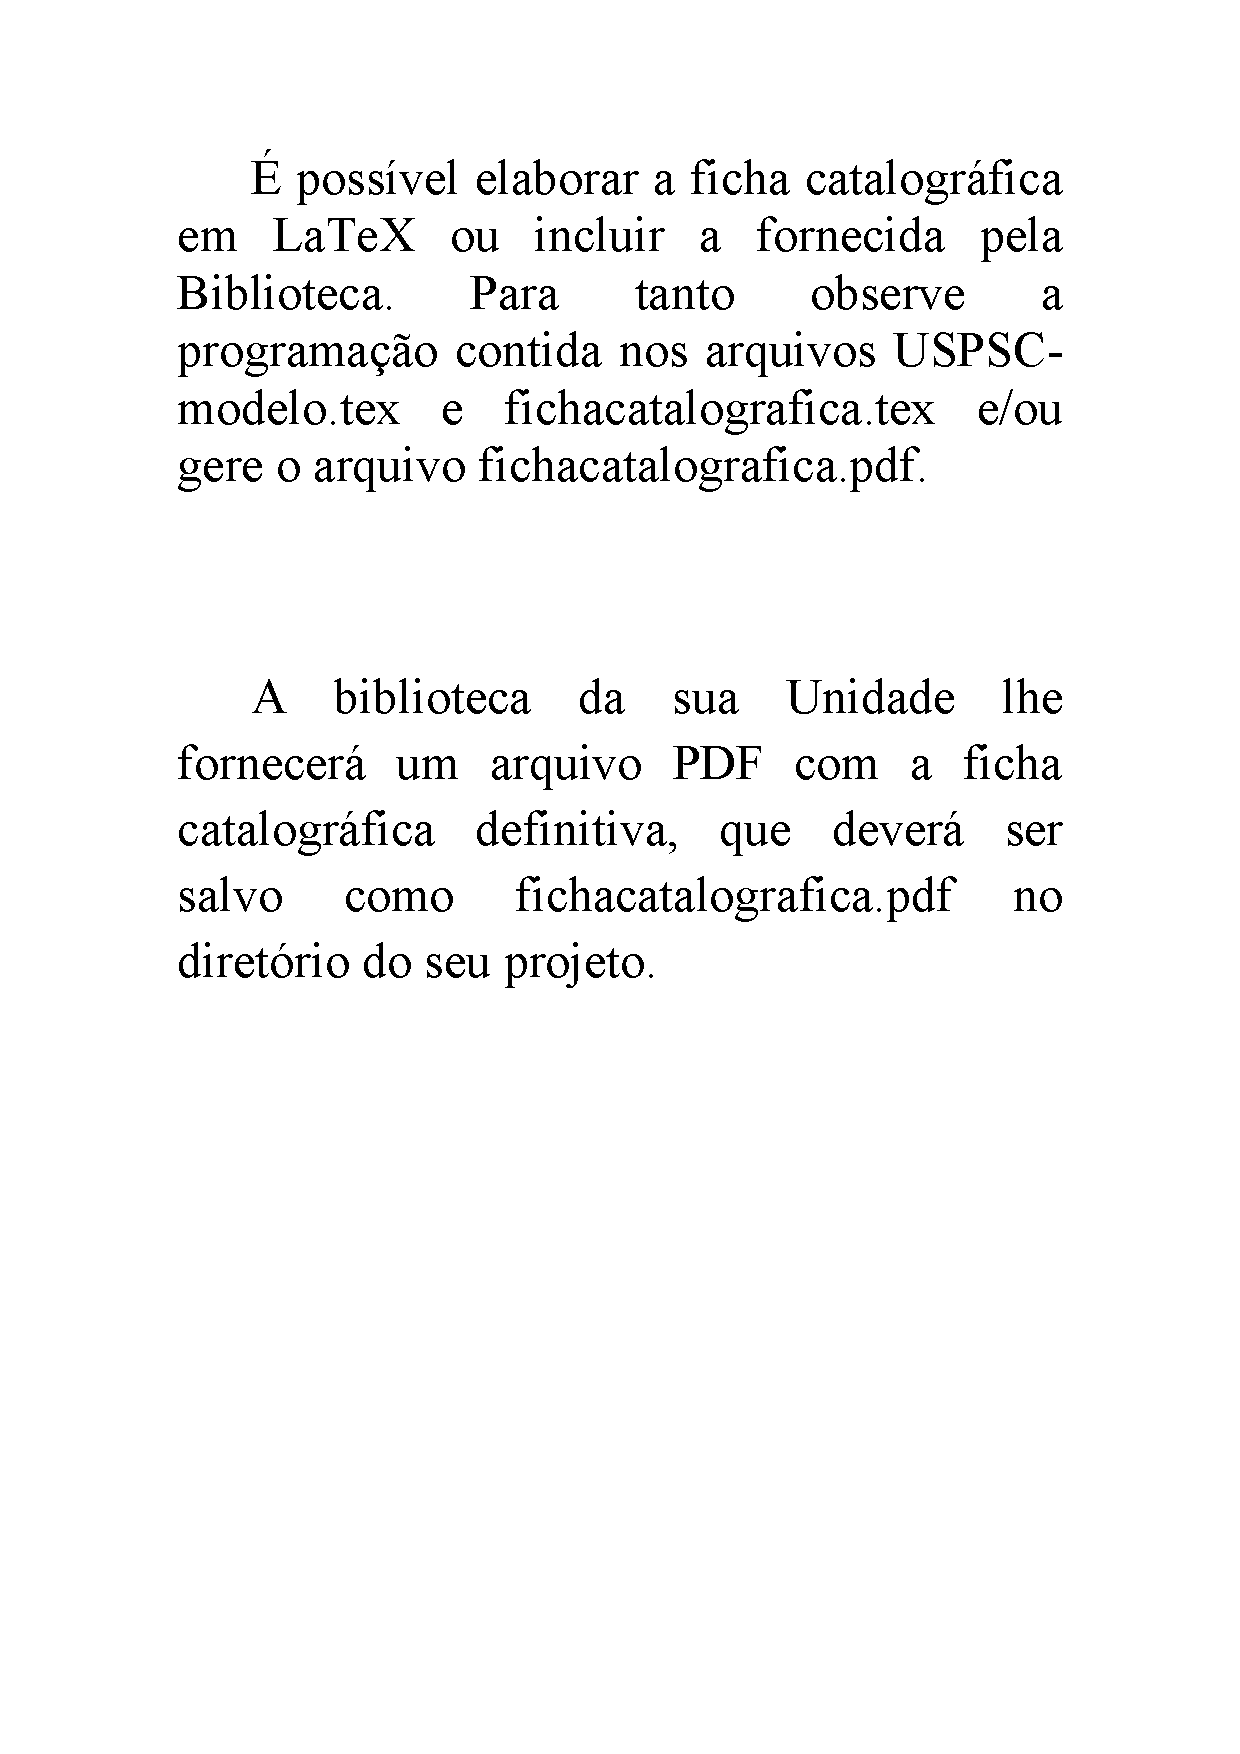
\includepdf{USPSC-TA-PreTextual/USPSC-fichacatalografica.pdf}

% Se você optar por elaborar a ficha catalográfica, deverá 
% incluir uma % antes da linha % antes
% do comando %% USPSC-fichacatalografica.tex
% ---
% Inserir a ficha bibliografica
% ---
% Isto é um exemplo de Ficha Catalográfica, ou ``Dados internacionais de
% catalogação-na-publicação''. Você pode utilizar este modelo como referência. 
% Porém, provavelmente a biblioteca da sua universidade lhe fornecerá um PDF
% com a ficha catalográfica definitiva após a defesa do trabalho. Quando estiver
% com o documento, salve-o como PDF no diretório do seu projeto e substitua todo
% o conteúdo de implementação deste arquivo pelo comando abaixo:
%
\begin{fichacatalografica}
	\hspace{-1.4cm}
	\imprimirnotaautorizacao \\ \\
	%\sffamily
	\vspace*{\fill}					% Posição vertical
\begin{center}					% Minipage Centralizado
  \imprimirnotabib \\
  \begin{table}[htb]
	\scriptsize
	\centering	
	\begin{tabular}{|p{0.9cm} p{8.7cm}|}
		\hline
	      & \\
		  &	  \imprimirautorficha     \\
		
		 \imprimircutter & 
							\hspace{0.4cm}\imprimirtitulo~  / ~\imprimirautor~ ;  ~\imprimirorientadorcorpoficha. -- 	\imprimirlocal, \imprimirdata.   \\
		
		  &  % Para incluir nota referente à versão corrigida no corpo da ficha,
			  % incluir % no início da linha acima e tirar a % do início da linha abaixo
			  %	\hspace{0.4cm} \imprimirtitulo~  / ~\imprimirautor~ ; ~\imprimirorientadorcorpoficha~- ~\imprimirnotafolharosto. -- \imprimirlocal, \imprimirdata.  \\
		
			\hspace{0.4cm}\pageref{LastPage} p. : il. (algumas color.) ; 30 cm.\\ 
		  & \\
		  & 
		    \hspace{0.4cm}\imprimirnotaficha ~--~ 
						  \imprimirunidademin, 
						  \imprimiruniversidademin, 
		                  \imprimirdata. \\ 
		  & \\                 
		   % Para incluir nota referente à versão corrigida em notas,
		    % incluir uma % no início da linha acima e	
		    % tirar a % do início da linha abaixo
		    % & \hspace{0.4cm}\imprimirnotafolharosto \\ 
		  & \\ 
		  & \hspace{0.4cm}1. LaTeX. 2. abnTeX. 3. Classe USPSC. 4. Editoração de texto. 5. Normalização da documentação. 6. Tese. 7. Dissertação. 8. Documentos (elaboração). 9. Documentos eletrônicos. I. \imprimirorientadorficha. 
		   II. Título. \\
	
		     %Se houver co-orientador, inclua % antes da linha (antes de II. Título.) 
		     %          e tire a % antes do comando abaixo 
		     %III. Título. \\   
		  \hline
	\end{tabular}
  \end{table}
\end{center}
\end{fichacatalografica}
% ---

 
% e retirar o % do comando abaixo
%%% USPSC-fichacatalografica.tex
% ---
% Inserir a ficha bibliografica
% ---
% Isto é um exemplo de Ficha Catalográfica, ou ``Dados internacionais de
% catalogação-na-publicação''. Você pode utilizar este modelo como referência. 
% Porém, provavelmente a biblioteca da sua universidade lhe fornecerá um PDF
% com a ficha catalográfica definitiva após a defesa do trabalho. Quando estiver
% com o documento, salve-o como PDF no diretório do seu projeto e substitua todo
% o conteúdo de implementação deste arquivo pelo comando abaixo:
%
\begin{fichacatalografica}
	\hspace{-1.4cm}
	\imprimirnotaautorizacao \\ \\
	%\sffamily
	\vspace*{\fill}					% Posição vertical
\begin{center}					% Minipage Centralizado
  \imprimirnotabib \\
  \begin{table}[htb]
	\scriptsize
	\centering	
	\begin{tabular}{|p{0.9cm} p{8.7cm}|}
		\hline
	      & \\
		  &	  \imprimirautorficha     \\
		
		 \imprimircutter & 
							\hspace{0.4cm}\imprimirtitulo~  / ~\imprimirautor~ ;  ~\imprimirorientadorcorpoficha. -- 	\imprimirlocal, \imprimirdata.   \\
		
		  &  % Para incluir nota referente à versão corrigida no corpo da ficha,
			  % incluir % no início da linha acima e tirar a % do início da linha abaixo
			  %	\hspace{0.4cm} \imprimirtitulo~  / ~\imprimirautor~ ; ~\imprimirorientadorcorpoficha~- ~\imprimirnotafolharosto. -- \imprimirlocal, \imprimirdata.  \\
		
			\hspace{0.4cm}\pageref{LastPage} p. : il. (algumas color.) ; 30 cm.\\ 
		  & \\
		  & 
		    \hspace{0.4cm}\imprimirnotaficha ~--~ 
						  \imprimirunidademin, 
						  \imprimiruniversidademin, 
		                  \imprimirdata. \\ 
		  & \\                 
		   % Para incluir nota referente à versão corrigida em notas,
		    % incluir uma % no início da linha acima e	
		    % tirar a % do início da linha abaixo
		    % & \hspace{0.4cm}\imprimirnotafolharosto \\ 
		  & \\ 
		  & \hspace{0.4cm}1. LaTeX. 2. abnTeX. 3. Classe USPSC. 4. Editoração de texto. 5. Normalização da documentação. 6. Tese. 7. Dissertação. 8. Documentos (elaboração). 9. Documentos eletrônicos. I. \imprimirorientadorficha. 
		   II. Título. \\
	
		     %Se houver co-orientador, inclua % antes da linha (antes de II. Título.) 
		     %          e tire a % antes do comando abaixo 
		     %III. Título. \\   
		  \hline
	\end{tabular}
  \end{table}
\end{center}
\end{fichacatalografica}
% ---


% As informações que compõem a ficha catalográfica estão 
% definidas no arquivo USPSC-pre-textual-UUUU.tex
% ---

% ---
% Folha de rosto adicional
% Para imprimir a folha de rosto adicional, exigida por algumas Unidades, a exemplo do ICMC,
% retire a % antes do comando abaixo

\imprimirfolhaderostoadic*

% ---
% ---
% Inserir errata
% ---

% %% USPSC-Errata.tex
\begin{errata}
	%\OnehalfSpacing 			
	A errata é um elemento opcional, que consiste de uma lista de erros da obra, precedidos pelas folhas e linhas onde eles ocorrem e seguidos pelas correções correspondentes. Deve ser inserida logo após a folha de rosto e conter a referência do trabalho para facilitar sua identificação, conforme a ABNT NBR 14724 \cite{nbr14724}.
	
	Modelo de Errata:
		
	\begin{flushleft} 
			\setlength{\absparsep}{0pt} % ajusta o espaçamento da referência	
			\SingleSpacing 
			\imprimirautorabr~ ~\textbf{\imprimirtituloresumo}.	\imprimirdata. \pageref{LastPage}p. 
			%Substitua p. por f. quando utilizar oneside em \documentclass
			%\pageref{LastPage}f.
			\imprimirtipotrabalho~-~\imprimirinstituicao, \imprimirlocal, \imprimirdata. 
 	\end{flushleft}
\vspace{\onelineskip}
\OnehalfSpacing 
\center
\textbf{ERRATA}
\vspace{\onelineskip}
\OnehalfSpacing 
\begin{table}[htb]
	\center
	\footnotesize
	\begin{tabular}{p{2cm} p{2cm} p{4cm} p{4cm} }
		\hline
		\textbf{Folha} & \textbf{Linha}  & \textbf{Onde se lê}  & \textbf{Leia-se}  \\
			\hline
			1 & 10 & auto-conclavo & autoconclavo\\
		\hline
	\end{tabular}
\end{table}
\end{errata}
% ---

% ---

% ---
% Inserir folha de aprovação
% ---

% A Folha de aprovação é um elemento obrigatório da NBR 4724/2011 (seção 4.2.1.3). 
% Após a defesa/aprovação do trabalho, gere o arquivo folhadeaprovacao.pdf da página assinada pela banca 
% e iclua o arquivo utilizando o comando abaixo:


% 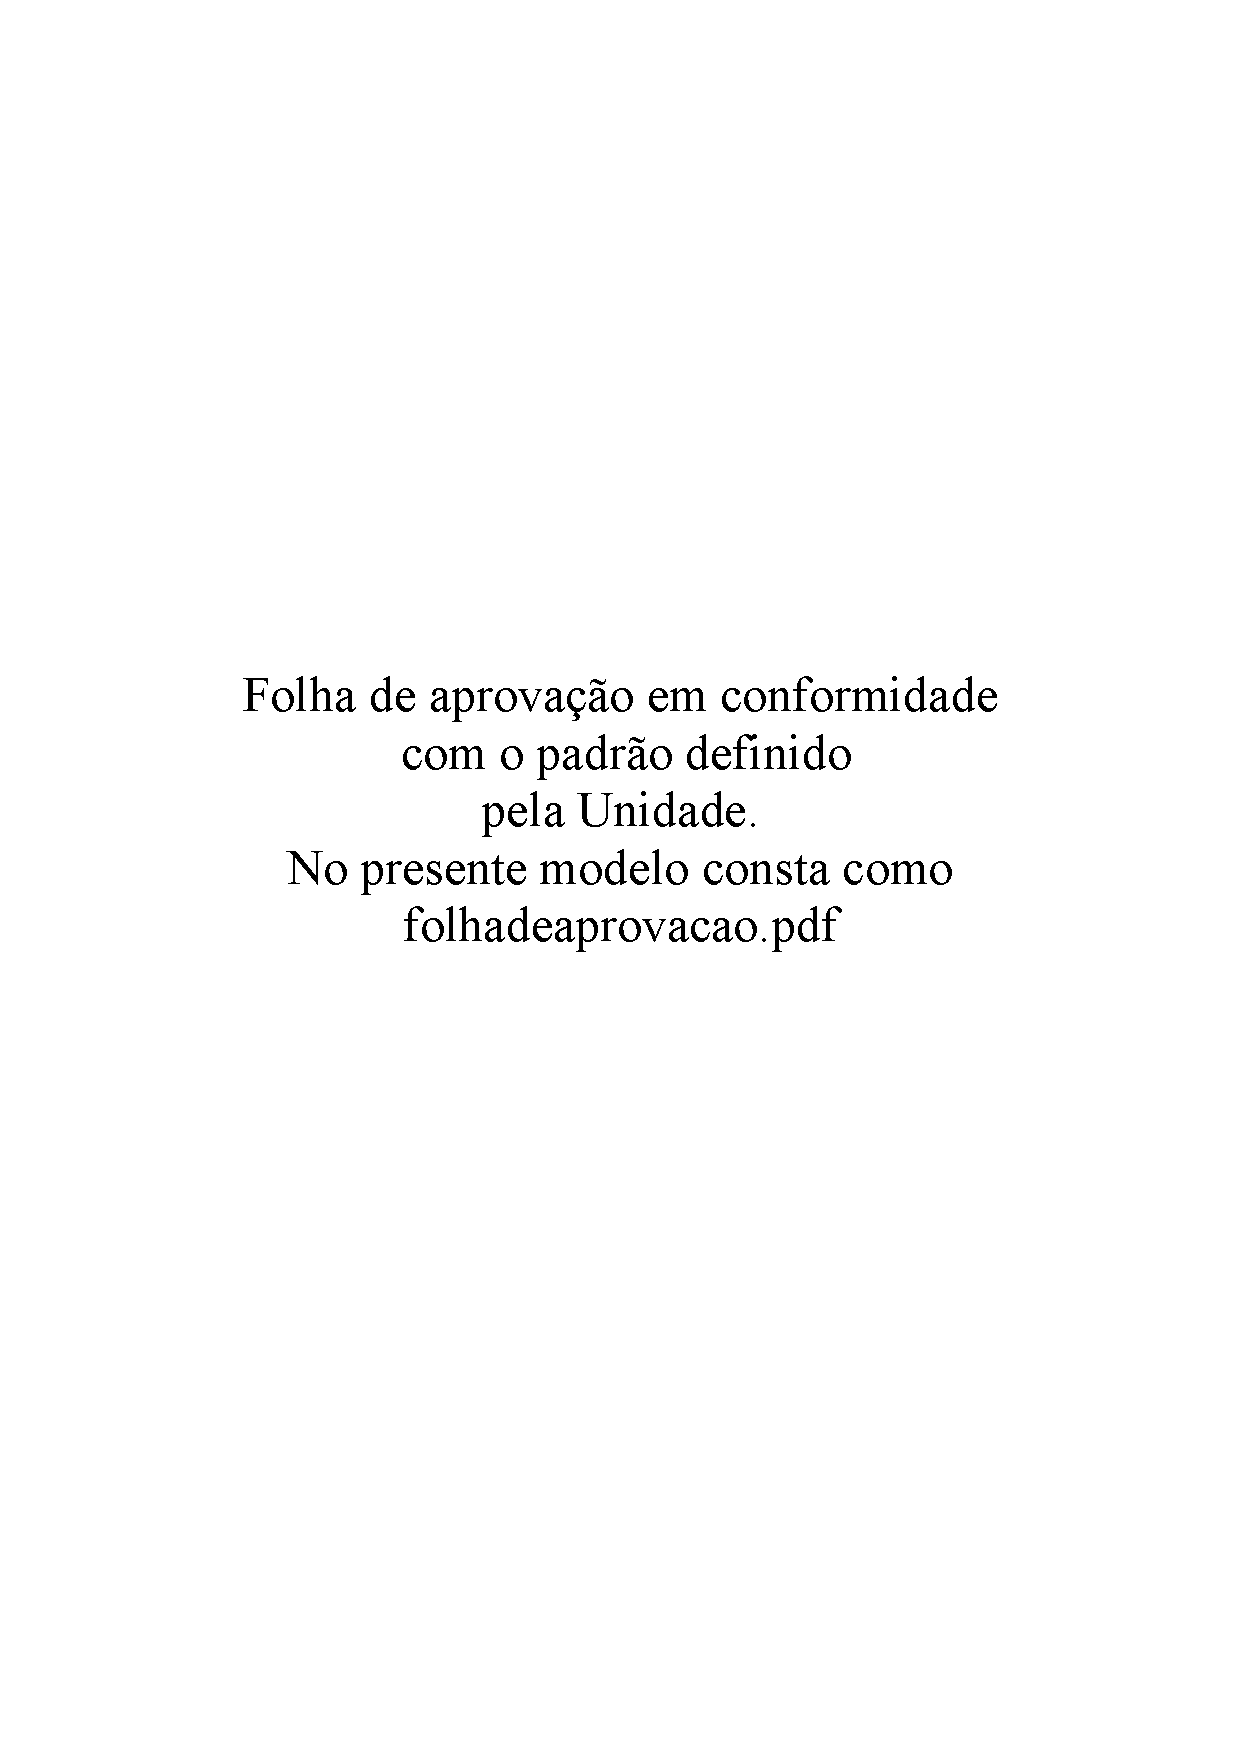
\includepdf{USPSC-TA-PreTextual/USPSC-folhadeaprovacao.pdf}


% Alternativa para a Folha de Aprovação:
% Se for a sua opção elaborar uma folha de aprovação, insira uma % antes do comando acima que inclui o arquivo folhadeaprovacao.pdf,
% tire o % do comando abaixo e altere o arquivo folhadeaprovacao.tex conforme suas necessidades
%\include{folhadeaprovacao}

\includepdf{USPSC-TA-PreTextual/USPSC-PaginaEmBranco.pdf}

% ---
% Dedicatória
% ---
% %% USPSC-Dedicatoria.tex
\begin{dedicatoria}
   \vspace*{\fill}
   \centering
   \noindent
   \textit{ Este trabalho é dedicado aos alunos da USP, como uma contribuição\\
  das Bibliotecas do Campus USP de São Carlos para o desenvolvimento\\
	e disseminação da pesquisa científica da Universidade.} \vspace*{\fill}
\end{dedicatoria}
% ---
% ---

% ---
% Agradecimentos
% ---
% %% USPSC-Agradecimentos.tex
\begin{agradecimentos}
	Primeira frase do agradecimento ....
	
	Segunda frase ....
	
	Outras frases ....
	
	Última frase ....
	
\end{agradecimentos}
% ---
% ---

% ---
% Epígrafe
% ---
% %% USPSC-Epigrafe.tex
\begin{epigrafe}
    \vspace*{\fill}
	\begin{flushright}
		\textit{``O estudo, a busca da verdade e da beleza são domínios \\
		em que nos é consentido sermos crianças por toda a vida.''\\
		Albert Einstein}
	\end{flushright}
\end{epigrafe}
% ---
% ---

% A T E N Ç Ã O
% Se o idioma do texto for em inglês, o abstract deve preceder o resumo
% resumo em português
%
% Resumo
% ---
% %% USPSC-Resumo.tex
\setlength{\absparsep}{18pt} % ajusta o espaçamento dos parágrafos do resumo		
\begin{resumo}
	\begin{flushleft} 
			\setlength{\absparsep}{0pt} % ajusta o espaçamento da referência	
			\SingleSpacing 
			\imprimirautorabr~~\textbf{\imprimirtituloresumo}.	\imprimirdata. \pageref{LastPage}p. 
			%Substitua p. por f. quando utilizar oneside em \documentclass
			%\pageref{LastPage}f.
			\imprimirtipotrabalho~-~\imprimirinstituicao, \imprimirlocal, \imprimirdata. 
 	\end{flushleft}
	\OnehalfSpacing 			
	Este trabalho tem como propósito a aplicação de modelos de aprendizado de máquina e técnicas de inteligência artificial explicável aos dados da Coordenação de Internações de Ribeirão Preto, Brasil, com o objetivo de predizer reinternações hospitalares. A metodologia abrangeu o treinamento e seleção de classificadores em três fases distintas, culminando na análise de importância de variáveis por meio do método SHAP. Os resultados indicam que pacientes solteiros, que ficaram internados por menos horas e são mais jovens, apresentam maior risco de reinternação. Variáveis sazonais, como o mês ou dia da semana de internação, também demonstraram grande influência na predição de reinternação. No entanto, as acurácias dos modelos permaneceram abaixo de 60\%, apontando para oportunidades de aprimoramento na performance preditiva. Alternativas foram sugeridas para futuras melhorias, como a expansão do conjunto de dados e a exploração de modelos mais complexos. Essas conclusões, além de orientar melhorias específicas neste contexto, fornecem uma sólida base para pesquisas futuras, não apenas nesta base de dados específica, mas como diretrizes para investigações similares em outras bases, contribuindo para avanços contínuos na predição de reinternações hospitalares.
	
	\vspace{\onelineskip}
	\noindent
	\textbf{Palavras-chave}: Inteligência Artificial Explicável. Aprendizado de Máquina. Reinternações Hospitalares. Serviços de Saúde Mental.
\end{resumo}
% ---

% Abstract
% ---
% %% USPSC-Abstract.tex
%\autor{Silva, M. J.}
\begin{resumo}[Abstract]
 \begin{otherlanguage*}{english}
	\begin{flushleft} 
		\setlength{\absparsep}{0pt} % ajusta o espaçamento dos parágrafos do resumo		
 		\SingleSpacing  		\imprimirautorabr~~\textbf{\imprimirtitleabstract}.	\imprimirdata.  \pageref{LastPage}p. 
		%Substitua p. por f. quando utilizar oneside em \documentclass
		%\pageref{LastPage}f.
		\imprimirtipotrabalhoabs~-~\imprimirinstituicao, \imprimirlocal, 	\imprimirdata. 
 	\end{flushleft}
	\OnehalfSpacing 
   This is the english abstract.

   \vspace{\onelineskip}
 
   \noindent 
   \textbf{Keywords}: LaTeX. USPSC class. Thesis. Dissertation. Conclusion course paper. 
 \end{otherlanguage*}
\end{resumo}

% ---

% ---
% inserir lista de figurass
% ---
% \pdfbookmark[0]{\listfigurename}{lof}
% \listoffigures*
% \cleardoublepage
% ---

% ---
% inserir lista de tabelas
% ---
% \pdfbookmark[0]{\listtablename}{lot}
% \listoftables*
% \cleardoublepage
% ---

% ---
% inserir lista de quadros
% ---
% \pdfbookmark[0]{\listofquadroname}{loq}
% \listofquadro*
% \cleardoublepage
% ---

% ---
% inserir lista de abreviaturas e siglas
% ---
% % USPSC-AbreviaturasSiglas.tex
\begin{siglas}
    \item[ABNT] Associação Brasileira de Normas Técnicas
    \item[abnTeX] ABsurdas Normas para TeX
	\item[IBGE] Instituto Brasileiro de Geografia e Estatística
	\item[LaTeX] Lamport TeX
	\item[USP] Universidade de São Paulo
	\item[USPSC] Campus USP de São Carlos
\end{siglas}

% ---

% ---
% inserir lista de símbolos
% ---
% % USPSC-Simbolos.tex
\begin{simbolos}
  \item[$ \Gamma $] Letra grega Gama
  \item[$ \Lambda $] Lambda
  \item[$ \zeta $] Letra grega minúscula zeta
  \item[$ \in $] Pertence
\end{simbolos}
% ---
% ---
% inserir o sumario
% ---
\pdfbookmark[0]{\contentsname}{toc}
\tableofcontents*
\cleardoublepage
% ---
% ----------------------------------------------------------
% ELEMENTOS TEXTUAIS
% ----------------------------------------------------------
\textual
% Os capítulos são inseridos como arquivos externos 

% Capítulo 1 - Introdução
% ---
%% USPSC-Introducao.tex

% ----------------------------------------------------------
% Introdução (exemplo de capítulo sem numeração, mas presente no Sumário)
% ----------------------------------------------------------
\chapter[Introdução]{Introdução}
\label{Introdução}

\section{Contextualização e Motivação}\label{sec-context}

Nos últimos anos, houve um aumento dramático na quantidade de dados criados e compartilhados através da internet. Grande parte desse conteúdo está disponível publicamente e sem custo, representando um suprimento virtualmente ilimitado de dados de treinamento para várias tarefas de modelagem estatística e rotulagem. Essa \q{enxurrada de dados} apresenta desafios significativos, mas também oportunidades revolucionárias para o desenvolvimento de sistemas baseados em dados \cite{SeltzerZ09}.

O crescente volume de dados gerados a partir dessas diversas fontes tem impulsionado uma popularização da inteligência artificial (IA), sobretudo com o uso de aprendizado de máquina, que, de forma sucinta, trata da criação de algoritmos que respondam e se adaptem automaticamente aos dados sem a necessidade de intervenção humana de forma contínua \cite{chiavegatto2015}. Aliado a ferramentas poderosas para o processamento massivo e paralelo de dados, esses avanços têm permitido tanto à indústria quanto à comunidade científica desenvolver modelos altamente eficazes e realizar análises mais sofisticadas. A adoção generalizada de técnicas de aprendizado de máquina tem se mostrado fundamental para desvendar o potencial dos dados disponíveis, resultando em descobertas inovadoras e aplicações transformadoras em diversas áreas, incluindo o setor de saúde \cite{mlaplicadosaude}.

O número de estudos médicos de IA cresceu de forma exponencial no período de 2005 a 2019 \cite{ShortGuide2020}, revelando o forte interesse da comunidade científica em buscar métodos cada vez mais eficazes para aprimorar o cuidado e a qualidade de vida dos pacientes. A aplicação de modelos preditivos de aprendizado de máquina possui um potencial significativo para auxiliar na tomada de decisões em diversas etapas do cuidado à saúde, principalmente no diagnóstico, intervenção e acompanhamento de problemas de saúde \cite{obermeyer2017}.

Na área da saúde, as decisões tomadas pelos sistemas de IA podem ter um impacto significativo na vida das pessoas. Se os usuários não conseguem compreender o processo de tomada de decisão, podem não confiar no sistema, chegando até a rejeitá-lo. Portanto, a capacidade de fornecer uma explicação sobre como e por que uma decisão específica foi feita tornou-se uma qualidade essencial em sistemas desse tipo \cite{WagnerBenedikt2021Ahpo}. Além disso, a explicabilidade também pode auxiliar os desenvolvedores na identificação e correção de erros ou viés nos sistemas de IA, tornando-os mais justos e precisos.

Diante desse contexto, este trabalho se propõe a avaliar diversos modelos de classificação com o objetivo de prever a reinternação hospitalar de pacientes, utilizando um conjunto de dados de cuidados de saúde mental coletados pelo sistema de informação da Coordenação de Internações em Ribeirão Preto, Brasil, de julho de 2012 a dezembro de 2017. A relevância deste tipo de trabalho se dá, pois, por meio dessas previsões, medidas preventivas podem ser adotadas antecipadamente, evitando a necessidade de reinternação e, consequentemente, reduzindo os custos hospitalares, visto que o custo médio das internações é significativamente maior que o custo médio dos atendimentos ambulatoriais \cite{cesconetto2008}. Além da predição, o estudo também utilizará técnicas de inteligência artificial explicável (do inglês: \textit{explainable artificial inteligence} - XAI) a fim de identificar quais variáveis estão mais associadas a casos de reinternação, fornecendo informações relevantes para o desenvolvimento de políticas e medidas preventivas mais eficazes.

A \autoref{img:fluxogeral} apresenta um fluxo geral deste trabalho:

\begin{figure}[H]
	\centering
	\caption{\label{img:fluxogeral}Fluxo geral do trabalho}
	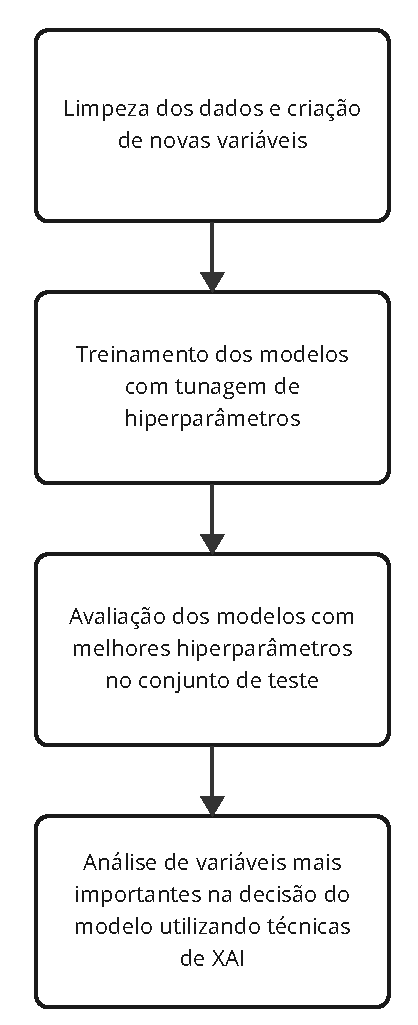
\includegraphics[scale=0.7]{USPSC-img/fluxo-geral-trabalho.pdf}
	\begin{center}
		Fonte: Autor (2023)
	\end{center}
\end{figure}
% ---

% ---
% Capítulo 2 - Revisão Bibliográfica
% ---
%% USPSC-Introducao.tex

% ----------------------------------------------------------
% Introdução (exemplo de capítulo sem numeração, mas presente no Sumário)
% ----------------------------------------------------------
\chapter[Revisão Bibliográfica]{Revisão Bibliográfica}
\label{Revisão}
Neste capítulo, serão apresentadas as fundamentações teóricas das técnicas de aprendizado de máquina utilizadas neste trabalho juntamente com um levantamento de estudos correlatos na área da saúde que empregaram técnicas semelhantes.

\section{Aprendizado de Máquina}
A crescente complexidade nos desafios computacionais e o volume massivo de dados gerados por diversas fontes impulsionaram a necessidade de ferramentas computacionais mais avançadas. Neste contexto, o aprendizado de máquina define-se como um campo de estudo da IA que dá aos computadores a habilidade de aprender sem serem explicitamente programados. Para tal, no aprendizado de máquina, os computadores são treinados para aprender com dados passados, utilizando técnicas que os possibilitem a derivar uma função ou hipótese capaz de solucionar problemas a partir de observações específicas, oferecendo soluções baseadas em dados históricos \cite{faceli}.

Os sistemas de aprendizado de máquina podem seguir vários paradigmas de aprendizado. Existem sistemas supervisionados, não supervisionados, semi-supervisionados, auto-supervisionados e de reforço. O aprendizado supervisionado é usado quando o modelo pode ser treinado com exemplos rotulados, enquanto o aprendizado não supervisionado é usado quando não há rótulos disponíveis. O aprendizado semi-supervisionado é uma combinação dos dois, enquanto o auto-supervisionado é usado quando o modelo pode ser treinado com exemplos gerados automaticamente. O aprendizado por reforço é usado quando o modelo pode aprender a tomar decisões com base em recompensas e punições \cite{geron2022hands}.

Dentro do paradigma de aprendizado supervisionado, os algoritmos podem ser usados em tarefas de classificação ou regressão. A classificação é usada para prever classes, enquanto a regressão é usada para prever valores. Por exemplo, a classificação pode ser usada para prever se um e-mail é spam ou não, enquanto a regressão pode ser usada para prever o preço de uma casa com base em suas características \cite{geron2022hands}.

A seguir será apresentada uma breve introdução aos modelos de classificação utilizados no desenvolvimento deste projeto.

\subsection{K-Vizinhos Mais Próximos}

O algoritmo K-Vizinhos Mais Próximos (ou KNN, do inglês \textit{K-Nearest Neighbors}) é um método de classificação que opera com base na proximidade dos vizinhos mais próximos de um ponto de dados. Quando um novo ponto de dados precisa ser classificado, o algoritmo encontra os \textit{k} pontos mais próximos a ele a partir do conjunto de dados de treinamento. Em seguida, ele classifica o novo ponto de dados com base na classe mais frequente entre esses \textit{k} vizinhos mais próximos.
O algoritmo KNN assume que todas as observações correspondem a pontos em um espaço n-dimensional e não requer um processo de aprendizado. Ele apenas prevê a categoria do novo ponto de dados com base nas categorias dos pontos conhecidos no momento da classificação \cite{Wang_2019}.

Os “vizinhos mais próximos” de uma instância são mensurados por métricas de distância, tais como a distância Euclidiana ou de Manhattan. A título de exemplo, será apresentada a distância Euclidiana, definida pela \autoref{eq:dist}:

\begin{equation}
\label{eq:dist}
    d(x, x') = \sqrt{\sum_{i=1}^{n} (x_i - x_i')^2}.
\end{equation}

\subsection{Regress\~ao Logística}

A regressão logística é um modelo estatístico usado para modelar a probabilidade de um evento ocorrer em termos de variáveis independentes \cite{logreg}. O modelo logístico é baseado na função logística, definida pela \autoref{eq:logreg}. Na \autoref{img:logreg}, é apresentado um exemplo da curva logística.

\begin{equation}
    \label{eq:logreg}
    f(z) = \frac{1}{1 + e^z}.
\end{equation}

De forma simplificada, o modelo logístico pode ser definido da seguinte maneira:

\begin{equation}
    \hat{y} = f(Z) = P(y = 1 | Z) = \frac{1}{1 + e^{-Z}}.
\end{equation}

onde $P(y = 1 | Z)$ é a probabilidade de ocorrência da classe positiva dado Z. Sendo Z:

\begin{equation}
    Z = \ln(\frac{p}{1 - p}) = \alpha + \sum_{j=1}^{k} \beta_k X_{ik}.
\end{equation}

onde \textit{p} representa a probabilidade de ocorrência do evento de interesse, enquanto \textit{X} denota o conjunto de variáveis preditoras. Os parâmetros do modelo, $\alpha$ e $\beta$, são estimados por meio da técnica de máxima verossimilhança \cite{favero}. Essa abordagem visa encontrar uma combinação de coeficientes que maximize a probabilidade de ocorrência do evento de interesse.

\begin{figure}
    \centering
    \caption{\label{img:logreg}Exemplo de função logística.}
    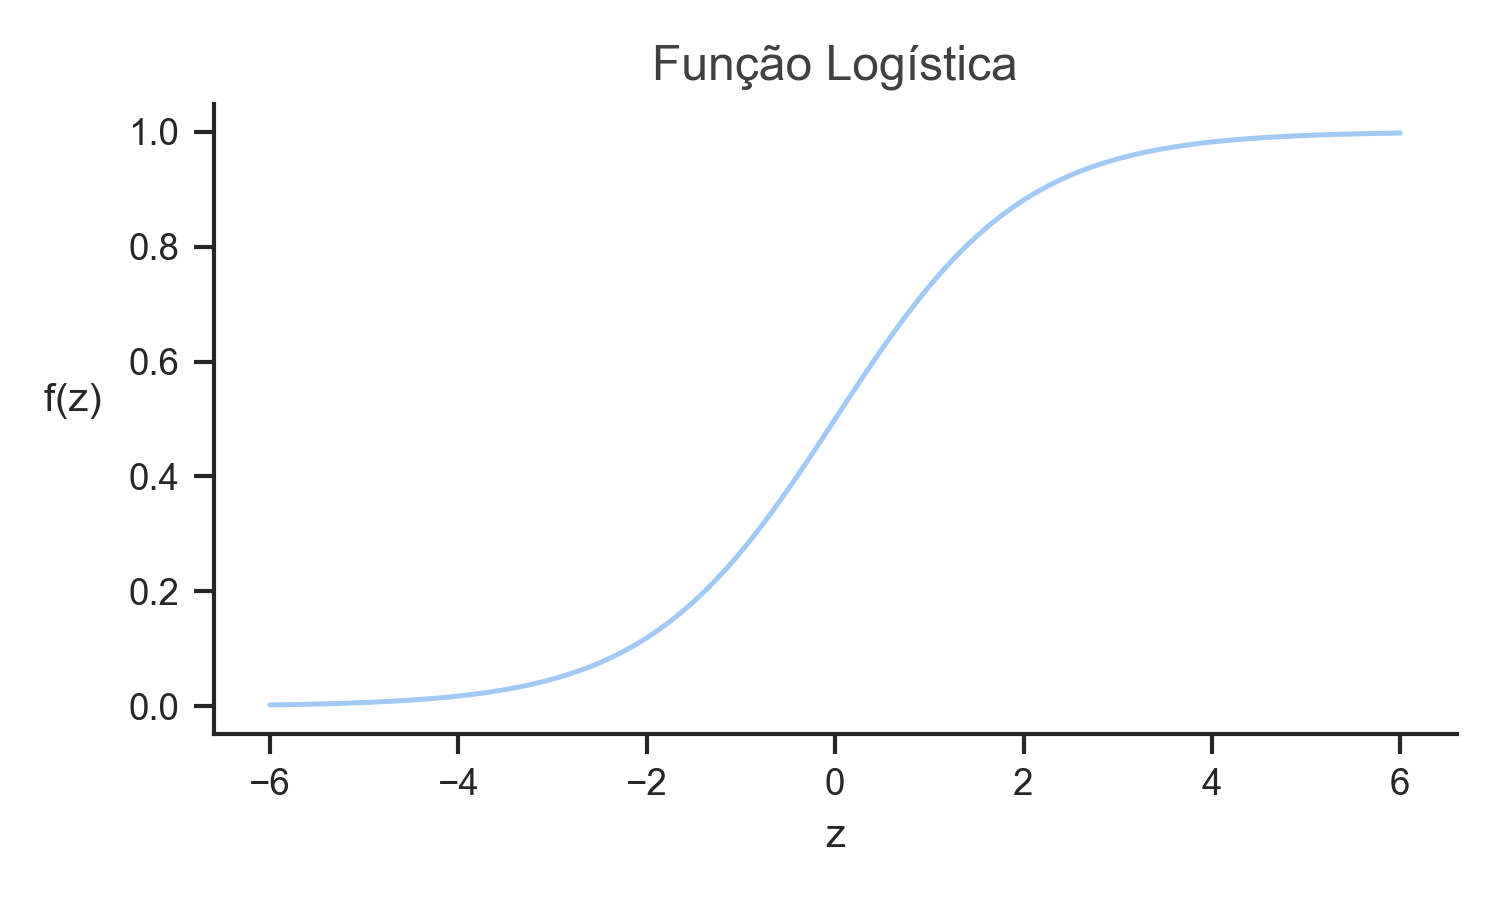
\includegraphics[scale=0.7]{USPSC-img/funcao-logistica.png}
    \begin{center}
        Fonte: Autor (2023).
    \end{center}
\end{figure}

\subsection{Máquinas de Vetores de Suporte}

As Máquinas de Vetores de Suporte, ou \textit{Support Vector Machines} (SVM), são um método de aprendizado supervisionado que busca encontrar o hiperplano de separação que maximiza a margem entre as classes. Elas são usadas em problemas de classificação para encontrar a melhor fronteira de decisão entre as classes, permitindo sobreposição entre elas, mas minimizando essa sobreposição. As SVMs são particularmente úteis em problemas de classificação com muitas características, onde outras técnicas podem sofrer de sobreajuste, o que as torna robustas em relação a ruídos e \textit{outliers} \cite{trevorHastie}.

As SVMs podem lidar com conjuntos de dados não lineares por meio do uso de \textit{kernels}, que mapeiam os dados para um espaço de maior dimensão onde eles podem ser separados linearmente. Na \autoref{img:kernelsvm}, é apresentado um exemplo de um espaço de características que foi transformado.

\begin{figure}[htb]
	\centering
	\caption{\label{img:kernelsvm}Exemplo de transformação utilizando \textit{kernel}: Convertendo um problema de classificação não linear em um problema de classificação linear em uma dimensão superior.}
	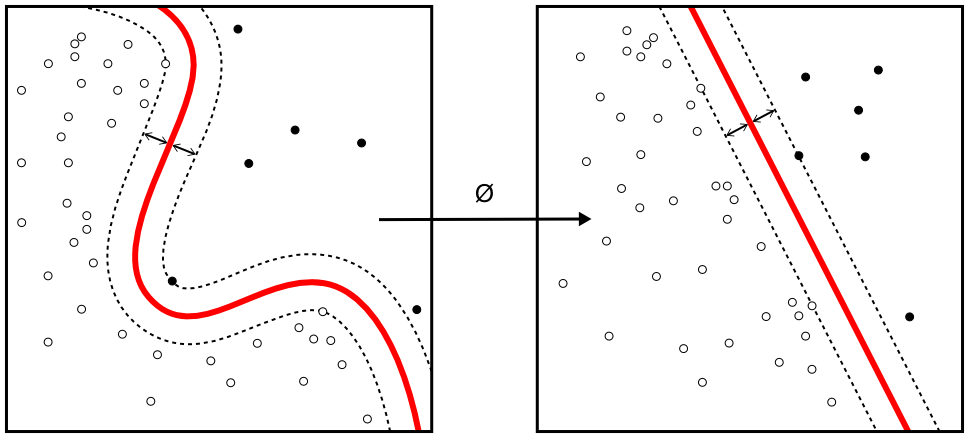
\includegraphics[scale=0.5]{USPSC-img/Kernel_Machine.png}
	\begin{center}
		Fonte: \cite{wiki}.
	\end{center}
\end{figure}

Embora as SVMs sejam amplamente utilizadas e tenham várias vantagens, também apresentam algumas desvantagens. Uma das principais desvantagens das SVMs é a necessidade de ajuste cuidadoso dos parâmetros do modelo, como o parâmetro de regularização e a escolha do \textit{kernel}, o que pode ser uma tarefa desafiadora e exigir conhecimento especializado. Além disso, as SVMs podem ser computacionalmente intensivas, especialmente em conjuntos de dados muito grandes, o que pode tornar seu treinamento demorado. Outra limitação das SVMs é a dificuldade em lidar com conjuntos de dados com muitas classes, uma vez que a abordagem de um-contra-um para problemas multiclasse pode levar a um grande número de classificadores binários \cite{trevorHastie}.

\subsection{Florestas Aleatórias e \textit{Gradient Boosted Trees}}

As Florestas Aleatórias (do inglês \textit{Random Forests}) e \textit{Gradient Boosted Trees} são exemplos de comitês (\textit{ensembles}) de algoritmos de aprendizado de máquina. Resumidamente, o método consiste na construção de múltiplas árvores de decisão em subespaços aleatórios do espaço de características, utilizando amostras aleatórias dos dados de treinamento e subconjuntos aleatórios das características disponíveis. Cada árvore de decisão é capaz de generalizar sua classificação de forma única, e a combinação das previsões de todas as árvores resulta em uma melhoria monotônica na precisão da classificação \cite{RandomForests}. Estudos recentes têm indicado que a aplicação desses algoritmos tem apresentado desempenho superior na previsão em comparação com outros métodos de aprendizado de máquina \cite{geron2022hands, Raschka}. Na \autoref{img:rfexample}, é ilustrada a construção de três árvores de decisão para um problema de classificação, construídas pelo algoritmo \textit{Random Forest}.

\begin{figure}
	\centering
	\caption{\label{img:rfexample}Ilustração do algoritmo \textit{Random Forest}.}
	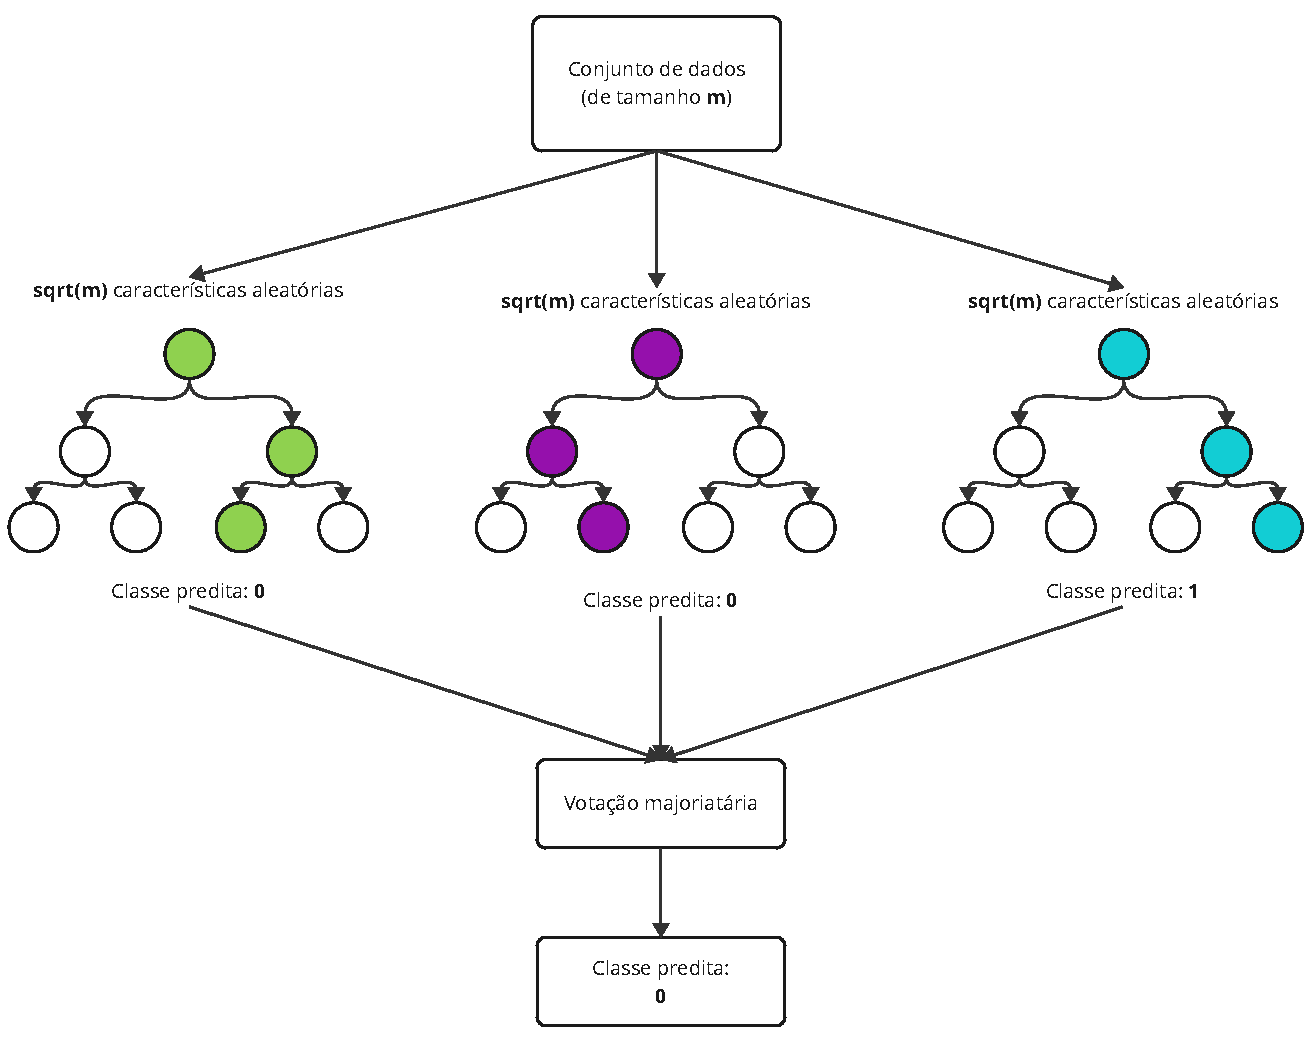
\includegraphics[scale=0.7]{USPSC-img/random_forest_example.pdf}
	\begin{center}
		Fonte: Adaptado de \citeonline{mlaplicadosaude}.
	\end{center}
\end{figure}

Com o objetivo de melhorar a precisão das previsões das árvores de decisão, o algoritmo \textit{Gradient Boosted Trees} \cite{friedman2000} utiliza a estratégia de \textit{boosting}. Em termos mais detalhados, o processo de \textit{boosting} geralmente começa com um modelo base simples, como uma árvore de decisão rasa. Este modelo é treinado no conjunto de dados e usado para fazer previsões. Em seguida, os exemplos que foram classificados incorretamente ou para os quais as previsões tiveram grandes erros são ponderados mais fortemente no próximo modelo a ser treinado. Este próximo modelo é treinado para se concentrar nos exemplos que foram mal classificados pelo modelo anterior, e o processo é repetido \cite{friedman2000}.

Ainda segundo \citeonline{friedman2000}, a técnica de \textit{Gradient Boosting} proposta pelo autor permitiu avanços importantes na capacidade de lidar com problemas complexos de previsão e classificação. Essa abordagem influenciou diretamente o desenvolvimento de algoritmos populares, como \textit{XGBoost} e \textit{LightGBM}, que são amplamente utilizados em competições de ciência de dados e em aplicações do mundo real devido à sua eficácia e desempenho.

\section{Inteligência Artificial Explicável}

A Inteligência Artificial Explicável refere-se à capacidade de compreender e explicar as decisões e previsões dos modelos de inteligência artificial. A explicabilidade é crucial para estabelecer a confiança do usuário, fornecer insights sobre como melhorar o modelo e compreender o processo que está sendo modelado. A capacidade de interpretar corretamente a saída de um modelo de previsão é extremamente importante, especialmente em contextos nos quais modelos complexos e de alto desempenho são utilizados \cite{Shap2017}. Nesta seção, será fornecida uma breve exposição do método de XAI aplicado neste trabalho, o \textit{SHapley Additive exPlanations} (SHAP).

\subsection{\textit{SHapley Additive exPlanations} (SHAP)}\label{sec:shap}

O SHAP \cite{Shap2017} unifica seis métodos existentes de interpretação de predições: LIME, DeepLIFT, Layer-wise Relevance Propagation (LRP), Shapley sampling values, SmoothGrad e Integrated Gradients.

O \textit{Local Interpretable Model-Agnostic Explanations} (LIME) \cite{Lime2016} é um método que explica as previsões de um modelo complexo construindo um modelo localmente interpretável em torno da previsão. O DeepLIFT \cite{Deeplift} compara a ativação de cada variável na previsão atual com a ativação média da variável em todas as previsões. O LRP \cite{LRP2015} atribui a importância de cada variável para uma previsão propagando a relevância da saída do modelo de volta para as entradas. O Shapley sampling values \cite{Strumbelj2014} amostra aleatoriamente subconjuntos de variáveis e calcula a contribuição média de cada variável para a previsão. O SmoothGrad \cite{SmoothGrad} suaviza as entradas do modelo para reduzir o ruído e, em seguida, calcula a importância de cada variável para uma previsão. O Integrated Gradients \cite{IntegratedGradients} integra a contribuição de cada variável para uma previsão ao longo de um caminho suave entre a entrada atual e uma entrada de referência.

O SHAP unifica esses métodos por meio da introdução do conceito de \q{modelo de explicação}, que representa uma aproximação interpretável do modelo original. Além disso, fornece resultados teóricos que asseguram a existência de uma solução única na classe de métodos aditivos, atendendo a um conjunto de propriedades desejáveis, incluindo consistência, localidade e completude. O SHAP propõe uma nova medida de importância de variáveis chamada \textit{SHAP value}, a única medida aditiva que satisfaz essas propriedades. Esses valores, conforme demonstrado pelo SHAP, estão alinhados com a intuição humana e são eficazes na discriminação entre classes de saída do modelo \cite{Shap2017}.

\section{Trabalhos de classificação na área médica}\label{sec-context}

A utilização de algoritmos de aprendizado de máquina para análises preditivas é uma tarefa que envolve uma série de etapas que vão desde  a preparação dos dados, até o lançamento e monitoramento da solução \cite{geron2022hands}. O trabalho de \citeonline{SantosHellenGeremiasdos2019Mlpa} se propõe a exemplificar as etapas envolvidas na utilização desses algoritmos para análises preditivas em saúde, com um exemplo de aplicação para predizer óbito em idosos de São Paulo. A metodologia empregada envolveu a utilização de diferentes algoritmos de aprendizado de máquina para treinar modelos preditivos a partir de dados do estudo SABE, e a avaliação desses modelos em termos de acurácia, sensibilidade e especificidade. Os resultados mostraram que os modelos tiveram desempenho razoável na predição de óbito em idosos, com destaque para o algoritmo Random Forest. No entanto, os autores ressaltam que a amostra utilizada foi relativamente pequena e que a performance dos modelos pode ser melhorada com mais dados e refinamento dos algoritmos.

O trabalho de \citeonline{LORETO2020103636} aborda a predição de reinternações em UTI usando algoritmos de classificação. A proposta é investigar se as características basais e informações coletadas no momento da admissão do paciente podem possibilitar previsões precisas de reinternação na UTI. A metodologia empregada envolveu a análise de um conjunto de dados de 11.805 pacientes adultos de três UTIs em um hospital universitário brasileiro, com a exclusão de pacientes falecidos durante a primeira admissão na UTI. Foram testados oito algoritmos de classificação e avaliados com base em seis métricas. Os resultados mostraram que as características do paciente registradas na admissão na UTI foram capazes de prever o risco de reinternação, superando modelos anteriores que utilizavam apenas dados disponíveis na alta da UTI.

\citeonline{WANG2021351} apresentam um estudo sobre a estimativa da probabilidade de reinternação à UTI para pacientes transferidos da UTI para a enfermaria geral, abordando os desafios de dados desbalanceados e esparsos. A pesquisa visa melhorar a gestão médica e reduzir as taxas de reinternação à UTI, levando a melhores resultados para os pacientes e redução de custos de saúde. A metodologia empregada inclui a análise de valores ausentes, o teste de razão de verossimilhança e a utilização de um modelo de floresta aleatória com decaimento de peso. Os resultados mostram que o modelo proposto supera outros métodos tradicionais em sete indicadores de desempenho diferentes.

O artigo de \citeonline{Stiglic2014} propõe uma abordagem para a classificação de reinternações pediátricas usando modelos de diferentes hospitais, permitindo alta performance e compreensibilidade dos resultados. A metodologia empregada é baseada em \textit{deep learning} e \textit{stacked generalization}, e foi avaliada usando dados de 54 hospitais na Califórnia para demonstrar as possibilidades de implantação em larga escala. Os resultados mostraram melhorias significativas no desempenho de classificação e interpretabilidade dos resultados.

O trabalho de \citeonline{CDCWound} tem como objetivo avaliar se a classificação de feridas do \textit{Centers for Disease Control and Prevention} (CDC) pode ser usada como um indicador de risco para reinternação hospitalar em 30 dias após a cirurgia. A metodologia empregada foi uma revisão retrospectiva de pacientes submetidos a cirurgias eletivas em um hospital universitário. Os resultados mostraram que a classificação de feridas do CDC foi um preditor significativo de reinternação hospitalar em 30 dias após a cirurgia. Os autores concluem que a classificação de feridas do CDC pode ser uma ferramenta útil para identificar pacientes com maior risco de reinternação hospitalar após a cirurgia.

\citeonline{fernandes2021multipurpose} apresentam uma abordagem multipropósito de aprendizado de máquina para prever o prognóstico negativo da COVID-19 em São Paulo, Brasil. O trabalho envolveu o treinamento de cinco algoritmos de aprendizado de máquina com dados estruturados de pacientes com COVID-19, utilizando técnicas de validação cruzada e otimização bayesiana. O objetivo era prever o risco de desenvolver condições críticas em pacientes com COVID-19. Os resultados mostraram que a abordagem proposta teve um desempenho satisfatório na previsão do prognóstico negativo da COVID-19, o que pode ajudar na tomada de decisões clínicas e na alocação efetiva de recursos de saúde.

O trabalho de \citeonline{genesdisease} propõe uma metodologia baseada em aprendizado de máquina para identificar genes relacionados a doenças complexas. O modelo de aprendizado de máquina proposto utiliza uma matriz de similaridade funcional entre genes para prever doenças genéticas complexas. Essa matriz é construída a partir de medidas de similaridade entre genes, como perfis de expressão gênica, redes de interação proteína-proteína e Gene Ontology. Em seguida, um classificador de aprendizado de máquina é treinado com essa matriz para identificar genes relevantes para a doença em questão. O modelo proposto foi avaliado em relação à sua capacidade de identificar genes relacionados ao Transtorno do Espectro Autista e mostrou melhorias significativas em relação a outros métodos de identificação de genes. Foi desenvolvido um fluxo de trabalho automatizado para tornar a metodologia acessível a pesquisadores sem conhecimento extenso em programação e aprendizado de máquina.

\citeonline{rosa_galdamez_souza_melo_villarinho_leal_2023} apresentam um estudo que utiliza técnicas de aprendizado de máquina para classificar fatores que influenciam a ocorrência de dermatites ocupacionais. A metodologia empregada envolveu a avaliação de diferentes algoritmos de aprendizado de máquina, a comparação dos resultados obtidos por cada técnica e a identificação dos fatores mais influentes na ocorrência da lesão ocupacional. Os resultados indicaram que todas as técnicas apresentaram acuracidade entre 55\% e 69,4\%, sensitividade entre 49,1\% e 80,7\% e especificidade entre 50\% e 66,7\%. Os fatores mais influentes identificados foram a exposição a produtos químicos, o uso de equipamentos de proteção individual inadequados e a falta de treinamento adequado.

\section{Técnicas de explicação aplicadas a trabalhos de classificação na área médica}\label{sec-context}

A explicabilidade já foi identificada como um fator chave para a adoção de sistemas de IA numa vasta gama de contextos \cite{doshivelez2017rigorous, lipton2017mythos, ribeiro2016modelagnostic}. No estudo conduzido por \citeonline{Abououf2023}, é apresentado um sistema de monitoramento de saúde que utiliza inteligência artificial para detectar e classificar eventos e anomalias médicas. A metodologia empregada envolve a utilização de um modelo de detecção de anomalias e eventos, um modelo de classificação e uma técnica de explicabilidade chamada \textit{KernelSHAP}. O sistema foi avaliado em um conjunto de dados de pacientes e obteve resultados promissores na detecção e classificação de eventos e anomalias médicas. Além disso, a técnica de explicabilidade permitiu que os médicos entendessem melhor as decisões tomadas pelo sistema de inteligência artificial.

Com o uso de técnicas de aprendizado profundo e transferência de aprendizado para detectar a COVID-19 a partir de radiografias de tórax, o estudo de \citeonline{BRUNESE2020105608} utiliza as camadas de ativação da rede, ou seja, as áreas da radiografia de tórax que o modelo considerou para gerar a predição, para fornecer explicabilidade sobre a predição. Ainda segundo os autores, isso pode representar uma sugestão para o radiologista localizar imediatamente as áreas da radiografia de tórax que podem ser de interesse. Os resultados mostraram que o modelo proposto alcançou uma acurácia de 98,08\% na detecção de COVID-19 em radiografias de tórax. O estudo também sugere que essa tecnologia pode ser usada como uma ferramenta de triagem para ajudar no diagnóstico da COVID-19 em configurações clínicas do mundo real.

No trabalho de \citeonline{KIM2022103677} foi desenvolvida uma técnica de previsão de mortalidade relacionada ao calor em uma unidade espacial detalhada dentro de uma cidade, utilizando um modelo baseado em floresta aleatória e a técnica de explicação SHAP. A metodologia empregada incluiu a coleta de dados meteorológicos, demográficos e socioeconômicos, pré-processamento de dados, divisão em conjuntos de treinamento e teste, construção do modelo, otimização de hiperparâmetros, avaliação de desempenho e interpretação dos resultados. Os resultados mostraram que o modelo proposto é capaz de prever com precisão a mortalidade relacionada ao calor em uma área específica da cidade de Daegu, na Coreia do Sul. A técnica SHAP permitiu uma interpretação global e local dos resultados, identificando as variáveis mais importantes para a previsão.

Também utilizando modelos SHAP, o trabalho de \citeonline{healthcare11070929} utiliza técnicas para prever a fertilidade masculina, com o intuito de melhorar a transparência, responsabilidade e explicabilidade de sete modelos de IA padrão da indústria. A metodologia empregada consistiu em coletar dados de pacientes com problemas de fertilidade masculina e aplicar os modelos de IA para prever a fertilidade. Em seguida, foram utilizadas técnicas de amostragem e validação cruzada para avaliar a robustez e estabilidade de cada modelo. Por fim, a técnica de XAI foi utilizada para explicar o desempenho de cada modelo e os resultados mostraram que o SHAP foi capaz de interpretar as previsões dos sistemas de IA e fornecer explicações claras e compreensíveis para os usuários.

% ---
% Capítulo 3 - Desenvolvimento
% ---
%% USPSC-Cap2-Desenvolvimento.tex 

% ---
% Este capítulo, utilizado por diferentes exemplos do abnTeX2, ilustra o uso de
% comandos do abnTeX2 e de LaTeX.
% ---

\chapter{Desenvolvimento}\label{cap-desenv}

Neste capítulo, será apresentada uma exposição ordenada e detalhada do desenvolvimento do presente trabalho. O início deste capítulo se dá com uma explanação da metodologia empregada, delineando os passos e abordagens utilizados para alcançar os objetivos propostos.

\section{Metodologia}\label{sec-metodologia}

\subsection{Definiç\~ao de domínio do problema}

O problema abordado neste estudo refere-se à previsão de reinternação hospitalar de pacientes que receberam cuidados de saúde mental no sistema de informação da Coordenação de Internações em Ribeirão Preto, Brasil, no período de julho de 2012 a dezembro de 2017. Este domínio envolve a aplicação de modelos de classificação de aprendizado de máquina em um conjunto de dados específico, com o propósito de antecipar eventos de reinternação hospitalar. Além disso, o estudo incorpora técnicas de inteligência artificial explicável, notadamente o SHapley Additive exPlanations (SHAP), para identificar e quantificar as variáveis que apresentam maior influência nos casos de reinternação, contribuindo assim para uma compreensão mais profunda dos fatores associados a esses eventos. A análise deste domínio visa aprimorar a capacidade de tomada de decisões e políticas de saúde, com ênfase na prevenção eficaz e na otimização dos recursos hospitalares.

\subsection{Dados}

O conjunto de dados empregado neste estudo já foi explorado em outras pesquisas \cite{barros2016, eHealth, FeatureSensitivity}. Ele abrange informações de 8.755 pacientes, com uma média de idade de 37,6 anos. As características do conjunto de dados englobam aspectos sociodemográficos, dados sobre internações hospitalares, diagnósticos, utilização de serviços médicos, informações de alta hospitalar e registros temporais, como datas de admissão, alta e óbito. A \autoref{tab:dados} descreve as variáveis utilizadas neste estudo.

\begin{table}[H]
	\IBGEtab{
		\caption{\label{tab:dados}Variáveis utilizadas do conjunto de dados}
	}
	{
		\begin{tabular}{ccc}
			\toprule
			Nome da variável & Tipo da variável \\
			\midrule \midrule
   			Arranjo docimiliar & Categórica \\
   			\midrule
			AVC & Booleana \\
			\midrule
			Convulsão & Booleana \\
			\midrule
			Dia da semana na 1\textsuperscript{a} internação & Numérica (inteira) \\
			\midrule
			Diabetes & Booleana \\
			\midrule
			Diagnóstico (CID10) & Categórica \\
			\midrule
			Doença infecto & Booleana \\
			\midrule
			Estado civil & Categórica \\
			\midrule
			Etnia & Categórica \\
			\midrule
			HAS & Booleana \\
			\midrule
			Idade na 1\textsuperscript{a} internação & Numérica (inteira) \\
			\midrule
			Mês da 1\textsuperscript{a} internação & Numérica (inteira) \\
			\midrule
			Problemas respiratórios & Booleana \\
			\midrule
			Quantidade de problemas na 1\textsuperscript{a} internação & Numérico (inteira) \\
			\midrule
			Sexo & Categórica \\
			\midrule
			Situação profissão & Categórica \\
			\midrule
			Tempo de internação (em horas) & Numérica (contínua) \\
			\midrule
			Traumatismo & Booleana \\
			\bottomrule
		\end{tabular}
	}
	{
		\fonte{Autor (2023)}
	}
\end{table}

É importante ressaltar que essas não são todas as variáveis disponíveis no conjunto de dados. Mais detalhes sobre como a seleção de atributos foi feita estão disponíveis na \autoref{sec:limpeza}.

\subsection{Ferramentas utilizadas}\label{sec:ferramentas}

É crescente o aumento da popularidade da linguagem Python em aplicações científicas.
Boa parte deste aumento se dá pela diversidade de bibliotecas científicas como Numpy e Scipy. Na área de Machine Learning, a linguagem Python apresenta diversas bibliotecas que permitem a execução de modelos de ML, com destaque para a biblioteca Scikit-Learn \cite{Buitinck}
%
%A proposta da biblioteca Scikit-Learn consiste em fornecer um conjunto de funcionalidades padronizadas, de modo a permitir que especialistas das mais diversas áreas
%possam construir modelos de Machine Learning (BUITINCK et al., 2013).
%Além de bem documentados, os modelos de ML implementados na biblioteca
%Scikit-Learn são padronizados quando ao input de dados e aos métodos disponíveis para
%a sua execução. Todos os modelos disponíveis na biblioteca aceitam entrada de dados na
%forma de arrays bidimensionais (observações x características).
%Há três componentes básicos: Transformer, Estimator e Predictor. Estes são apresentados a seguir, em conjunto com a Figura 1.13, a qual apresenta como estes componentes estão relacionados entre si e como são aplicados aos conjuntos de treinamento e de
%teste na busca pelo ajuste de modelos de Machine Learning. Pressupõe-se que o conjunto
%de dados foi dividido em duas partes: treinamento e teste, para o qual a biblioteca ScikitLearn dispõe do método train_test_split, que pode ser utilizado como segue:

\subsection{Limpeza, análise exploratória e prepação dos dados}\label{sec:limpeza}

Inicialmente, a limpeza dos dados será realizada para garantir a consistência e integridade do conjunto de dados. Em seguida, uma análise exploratória detalhada dos dados será conduzida, com a possibilidade de criação de novas variáveis que possam proporcionar insights valiosos. Um exemplo é a variável "tempo de internação", definida como a diferença entre a data de entrada e a data de saída, que poderá ser criada para uma compreensão mais precisa do tempo de permanência dos pacientes.

\subsection{Treinamento dos classificadores}

Posteriormente, a fase de treinamento dos classificadores será iniciada, explorando diferentes algoritmos de aprendizado de máquina, ajustando seus hiperparâmetros e empregando a validação cruzada para garantir que os modelos sejam robustos e generalizáveis.

\subsection{Análise de variáveis mais importantes}
Por fim, será utilizada a biblioteca \texttt{shap} para avaliar o impacto das variáveis no processo de tomada de decisões dos modelos. Isso permitirá a identificação de quais características estão mais fortemente associadas a casos de reinternação hospitalar, fornecendo uma visão detalhada das relações entre variáveis e resultados.

\subsection{Apresentação dos resultados}
Os resultados obtidos após o término dos processos mencionados na seção TAL serão apresentados de maneira clara e concisa, utilizando tabelas e gráficos informativos. As tabelas destacarão métricas de desempenho, como precisão, recall, F1-score e área sob a curva ROC, para cada modelo testado. Além disso, serão fornecidos gráficos que ilustrarão a importância relativa das variáveis no processo de previsão, com base nas análises SHAP.

[Incluir imagem com o fluxograma do processo descrito na metodologia]


% Este capítulo é parte principal do trabalho acadêmico e deve conter a exposição ordenada e detalhada do assunto. Divide-se em seções e subseções, em conformidade com a abordagem do tema e do método, abrangendo: revisão bibliográfica, materiais e métodos, técnicas utilizadas, resultados obtidos e discussão.

% Abaixo são apresentados minimamente exemplos tabelas, quadros, divisões de documentos e outros itens. Consulte o \textbf{Tutorial do Pacote USPSC para modelos de trabalhos de acad\^emicos em LaTeX - vers\~ao 3.1} para demais informações. 

% \section{Resultados de comandos}\label{sec-divisoes}

% % ---
% \subsection{Tabelas e quadros}

% O \textbf{Tutorial do Pacote USPSC para modelos de trabalhos de acad\^emicos em LaTeX - vers\~ao 3.1} apresenta orientações completas e diversas formatações de tabelas, dentre elas a \autoref{tab-ibge}, que é um exemplo de tabela alinhada que pode ser longa ou curta, conforme padrão do Instituto Brasileiro de Geografia e Estatística (IBGE).

% %\begin{table}[H]
% \begin{table}[htb]
% 	\IBGEtab{%
% 		\caption{Frequência anual por categoria de usuários}%
% 		\label{tab-ibge}
% 	}{%
% 		\begin{tabular}{ccc}
% 			\toprule
% 			Categoria de Usuários & Frequência de Usuários \\
% 			\midrule \midrule
% 			Graduação & 72\% \\
% 			\midrule 
% 			Pós-Graduação & 15\% \\
% 			\midrule 
% 			Docente & 10\% \\
% 			\midrule 
% 			Outras & 3\% \\
% 			\bottomrule
% 		\end{tabular}%
% 	}{%
% 		\fonte{Elaborada pelos autores.}%
% 		\nota{Exemplo de uma nota.}%
% 		\nota[Anotações]{Uma anotação adicional, que pode ser seguida de várias
% 			outras.}%
		
% 	}
% \end{table}


% A formatação do quadro é similar à tabela, mas deve ter suas laterais fechadas e conter as linhas horizontais.
% \newpage

% % o comando \newpage foi utilizado para forçar a quebra de página

% \begin{quadro}[htb]
% 	\caption{\label{quadro_modelo}Níveis de investigação}
% 	\begin{tabular}{|p{2.6cm}|p{6.0cm}|p{2.25cm}|p{3.40cm}|}
% 		\hline
% 		\textbf{Nível de Investigação} & \textbf{Insumos}  & \textbf{Sistemas de Investigação}  & \textbf{Produtos}  \\
% 		\hline
% 		Meta-nível & Filosofia\index{filosofia} da Ciência  & Epistemologia &
% 		Paradigma  \\
% 		\hline
% 		Nível do objeto & Paradigmas do metanível e evidências do nível inferior &
% 		Ciência  & Teorias e modelos \\
% 		\hline
% 		Nível inferior & Modelos e métodos do nível do objeto e problemas do nível inferior & Prática & Solução de problemas  \\
% 		\hline
% 	\end{tabular}
% 	\begin{flushleft}
% 		%\fonte{\citeonline{van1986}}
% 		Fonte: \citeonline{}
% 	\end{flushleft}
% \end{quadro} 


% No \textbf{Tutorial do Pacote USPSC para modelos de trabalhos de acad\^emicos em LaTeX - vers\~ao 3.1} são apresentados mais exemplos de quadros.

% % ---
% \subsection{Figuras}\label{sec_figuras}
% % ---
% \index{figuras}Figuras podem ser criadas diretamente em \LaTeX,
% como o exemplo da \autoref{fig_circulo}. \\ 

% \begin{figure}[htb]
% 	\caption{\label{fig_circulo}A delimitação do espaço}
% 	\begin{center}
% 		\setlength{\unitlength}{9cm}
% 		\begin{picture}(1,1)
% 		\put(0,0){\line(0,1){1}}
% 		\put(0,0){\line(1,0){1}}
% 		\put(0,0){\line(1,1){1}}
% 		\put(0,0){\line(1,2){.5}}
% 		\put(0,0){\line(1,3){.3333}}
% 		\put(0,0){\line(1,4){.25}}
% 		\put(0,0){\line(1,5){.2}}
% 		\put(0,0){\line(1,6){.1667}}
% 		\put(0,0){\line(2,1){1}}
% 		\put(0,0){\line(2,3){.6667}}
% 		\put(0,0){\line(2,5){.4}}
% 		\put(0,0){\line(3,1){1}}
% 		\put(0,0){\line(3,2){1}}
% 		\put(0,0){\line(3,4){.75}}
% 		\put(0,0){\line(3,5){.6}}
% 		\put(0,0){\line(4,1){1}}
% 		\put(0,0){\line(4,3){1}}
% 		\put(0,0){\line(4,5){.8}}
% 		\put(0,0){\line(5,1){1}}
% 		\put(0,0){\line(5,2){1}}
% 		\put(0,0){\line(5,3){1}}
% 		\put(0,0){\line(5,4){1}}
% 		\put(0,0){\line(5,6){.8333}}
% 		\put(0,0){\line(6,1){1}}
% 		\put(0,0){\line(6,5){1}}
% 		\end{picture}
% 	\end{center}
% 	\legend{Fonte: \citeonline{equipeabntex2}}
% \end{figure}

% Consulte o \textbf{Tutorial do Pacote USPSC para modelos de trabalhos de acad\^emicos em LaTeX - vers\~ao 3.1} para conhecer mais recursos referentes à figuras. 

% % ---
% \section{Divisões do documento}\label{sec-divisoes-b}
% Esta seção exemplifica o uso de divisões de documentos em conformidade com a ABNT NBR 6024  \cite{nbr6024}.
% % ---
% % ---
% \subsection{Divisões do documento: subseção}\label{sec-divisoes-subsection}
% % ---

% Um exemplo de seção é a \autoref{sec-divisoes-b}. Esta é a \autoref{sec-divisoes-subsection}.

% \subsubsection{Divisões do documento: subsubseção}\label{sec-divisoes-subsubsection}

% Isto é uma \texttt{subsubsection} do \LaTeX, mas é denominada de ``subseção'' porque no português não temos a palavra ``subsubseção''.

% \subsubsection{Divisões do documento: subsubseção}

% Isto é outra subsubseção.

% \subsection{Divisões do documento: subseção}\label{sec-exemplo-subsec}

% Isto é uma subseção.

% \subsubsection{Divisões do documento: subsubseção}

% Isto é mais uma subsubseção da \autoref{sec-exemplo-subsec}.


% \subsubsubsection{Esta é uma subseção de quinto
% nível}\label{sec-exemplo-subsubsubsection}

% Esta é uma seção de quinto nível. Ela é produzida com o seguinte comando:

% \begin{verbatim}
% \subsubsubsection{Esta é uma subseção de quinto
% nível}\label{sec-exemplo-subsubsubsection}
% \end{verbatim}

% \subsubsubsection{Esta é outra subseção de quinto nível}\label{sec-exemplo-subsubsubsection-outro}

% Esta é outra seção de quinto nível.


% \paragraph{Este é um parágrafo numerado}\label{sec-exemplo-paragrafo}

% Este é um exemplo de parágrafo nomeado. Ele é produzido com o comando de
% parágrafo:

% \begin{verbatim}
% \paragraph{Este é um parágrafo nomeado}\label{sec-exemplo-paragrafo}
% \end{verbatim}

% A numeração entre parágrafos numerados e subsubsubseções são contínuas.

% \paragraph{Esta é outro parágrafo numerado}\label{sec-exemplo-paragrafo-outro}

% Este é outro parágrafo nomeado.

% % ---
% \subsection{Este é um exemplo de nome de subseção longa que se aplica a seções e demais divisões do documento. Ele deve estar alinhado à esquerda e a segunda e demais linhas devem iniciar logo abaixo da primeira palavra da primeira linha} 

% Observe que o alinhamento do título obedece esta regra também no sumário.
	








% Capítulo 4 - Conclusão
% ---
% \include{USPSC-TA-Textual/USPSC-Cap3-Conclusao}
% ---

% ----------------------------------------------------------
% ELEMENTOS PÓS-TEXTUAIS
% ----------------------------------------------------------
\postextual
% ----------------------------------------------------------

% -----------------------------------------------------------
% Referências bibliográficas
% ----------------------------------------------------------
\bibliography{USPSC-bib/USPSC-modelo-references}


% ----------------------------------------------------------
% Glossário
% ----------------------------------------------------------
%
% Consulte o manual da classe abntex2 para orientações sobre o glossário.
%
%\glossary

% ----------------------------------------------------------
% Apêndices
% ----------------------------------------------------------
% %% USPSC-Apendice.tex
% ---
% Inicia os apêndices
% ---

\begin{apendicesenv}
% Imprime uma página indicando o início dos apêndices
\partapendices
\chapter{Apêndice(s)}
Elemento opcional, que consiste em texto ou documento elaborado pelo autor, a fim de complementar sua argumentação, conforme a ABNT NBR 14724 \cite{nbr14724}.

Os apêndices devem ser identificados por letras maiúsculas consecutivas, seguidas de hífen e pelos respectivos títulos. Excepcionalmente, utilizam-se letras maiúsculas dobradas na identificação dos apêndices, quando esgotadas as 26 letras do alfabeto. A paginação deve ser contínua, dando seguimento ao texto principal. \cite{aguia2020}
% ----------------------------------------------------------
\chapter{Exemplo de tabela centralizada verticalmente e horizontalmente}
\index{tabelas}A \autoref{tab-centralizada} exemplifica como proceder para obter uma tabela centralizada verticalmente e horizontalmente.
% utilize \usepackage{array} no PREAMBULO (ver em USPSC-modelo.tex) obter uma tabela centralizada verticalmente e horizontalmente
\begin{table}[htb]
\ABNTEXfontereduzida
\caption[Exemplo de tabela centralizada verticalmente e horizontalmente]{Exemplo de tabela centralizada verticalmente e horizontalmente}
\label{tab-centralizada}

\begin{tabular}{ >{\centering\arraybackslash}m{6cm}  >{\centering\arraybackslash}m{6cm} }
\hline
 \centering \textbf{Coluna A} & \textbf{Coluna B}\\
\hline
  Coluna A, Linha 1 & Este é um texto bem maior para exemplificar como é centralizado verticalmente e horizontalmente na tabela. Segundo parágrafo para verificar como fica na tabela\\
  Quando o texto da coluna A, linha 2 é bem maior do que o das demais colunas  & Coluna B, linha 2\\
\hline
\end{tabular}
\begin{flushleft}
		Fonte: Elaborada pelos autores.\
\end{flushleft}
\end{table}

% ----------------------------------------------------------
\chapter{Exemplo de tabela com grade}
\index{tabelas}A \autoref{tab-grade} exemplifica a inclusão de traços estruturadores de conteúdo para melhor compreensão do conteúdo da tabela, em conformidade com as normas de apresentação tabular do IBGE.
% utilize \usepackage{array} no PREAMBULO (ver em USPSC-modelo.tex) obter uma tabela centralizada verticalmente e horizontalmente
\begin{table}[htb]
\ABNTEXfontereduzida
\caption[Exemplo de tabelas com grade]{Exemplo de tabelas com grade}
\label{tab-grade}
\begin{tabular}{ >{\centering\arraybackslash}m{8cm} | >{\centering\arraybackslash}m{6cm} }
\hline
 \centering \textbf{Coluna A} & \textbf{Coluna B}\\
\hline
  A1 & B1\\
\hline
  A2 & B2\\
\hline
  A3 & B3\\
\hline
  A4 & B4\\
\hline
\end{tabular}
\begin{flushleft}
		Fonte: Elaborada pelos autores.\
\end{flushleft}
\end{table}


\end{apendicesenv}
% ---

% ----------------------------------------------------------
% Anexos
% ----------------------------------------------------------
% %% USPSC-Anexos.tex
% ---
% Inicia os anexos
% ---
\begin{anexosenv}

% Imprime uma página indicando o início dos anexos
\partanexos

% ---
\chapter{Exemplo de anexo}
% ---
Elemento opcional, que consiste em um texto ou documento não elaborado pelo autor, que serve de fundamentação, comprovação e ilustração, conforme a ABNT NBR 14724. \cite{nbr14724}.

O \textbf{ANEXO B} exemplifica como incluir um anexo em pdf.

\chapter{Acentuação (modo texto - \LaTeX)}
\begin{figure}[H]
	\begin{center}
	\caption{\label{fig_anexob}Acentuação (modo texto - \LaTeX)}
	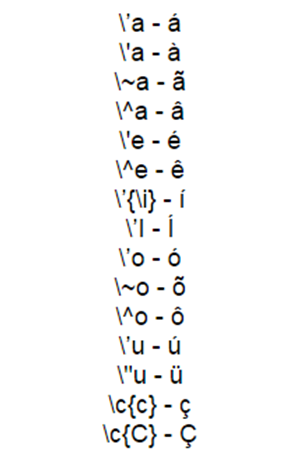
\includegraphics[scale=1.0]{USPSC-img/USPSC-AcentuacaoLaTeX.png} \\
	Fonte: \citeonline{comandos}
	\end{center}	
\end{figure}

\end{anexosenv}


%---------------------------------------------------------------------
% INDICE REMISSIVO
%--------------------------------------------------------------------
% %% USPSC-IndicexRemissivosTutorial.tex
% ---
% Inicia os Índices Remissivos
% ---
%---------------------------------------------------------------------
% INDICE REMISSIVO
%--------------------------------------------------------------------
\phantompart
\printindex
%---------------------------------------------------------------------


%---------------------------------------------------------------------

\end{document}
